\documentclass[.../Dokumentation.tex]{subfiles}
\begin{document}
\subsection{Fahrzeuge}\label{sec-ita4-cars}
Da die vorangegangene Iteration \ref{sec-ita3} gezeigt hat, dass auch ohne 
Stützmaterial kein zufriedenstellendes Ergebnis erzielt werden kann, 
wurde der Versuch unternommen, ein alternative Befestigungslösung zu erarbeiten. 
Die dem Druck mit Stützmaterial zugrunde liegende Problematik äußert sich in 
den horizontal durch das Fahrzeug geführten Hohlräumen für die Bolzen.\\
Deshalb wurde der Versuch unternommen, diese nun vertikal anzubringen.
Darüber hinaus sollte zusätzliche Stabilität in Längsrichtung gewonnen werden, 
indem eine Vorrichtung zum "einhängen" geschaffen wird. 
Beides ist in den Abbildungen \ref{fig-new-fixture-upper} und 
\ref{fig-new-fixture-lower} zu sehen.
\begin{figure}[H]
\begin{center}
    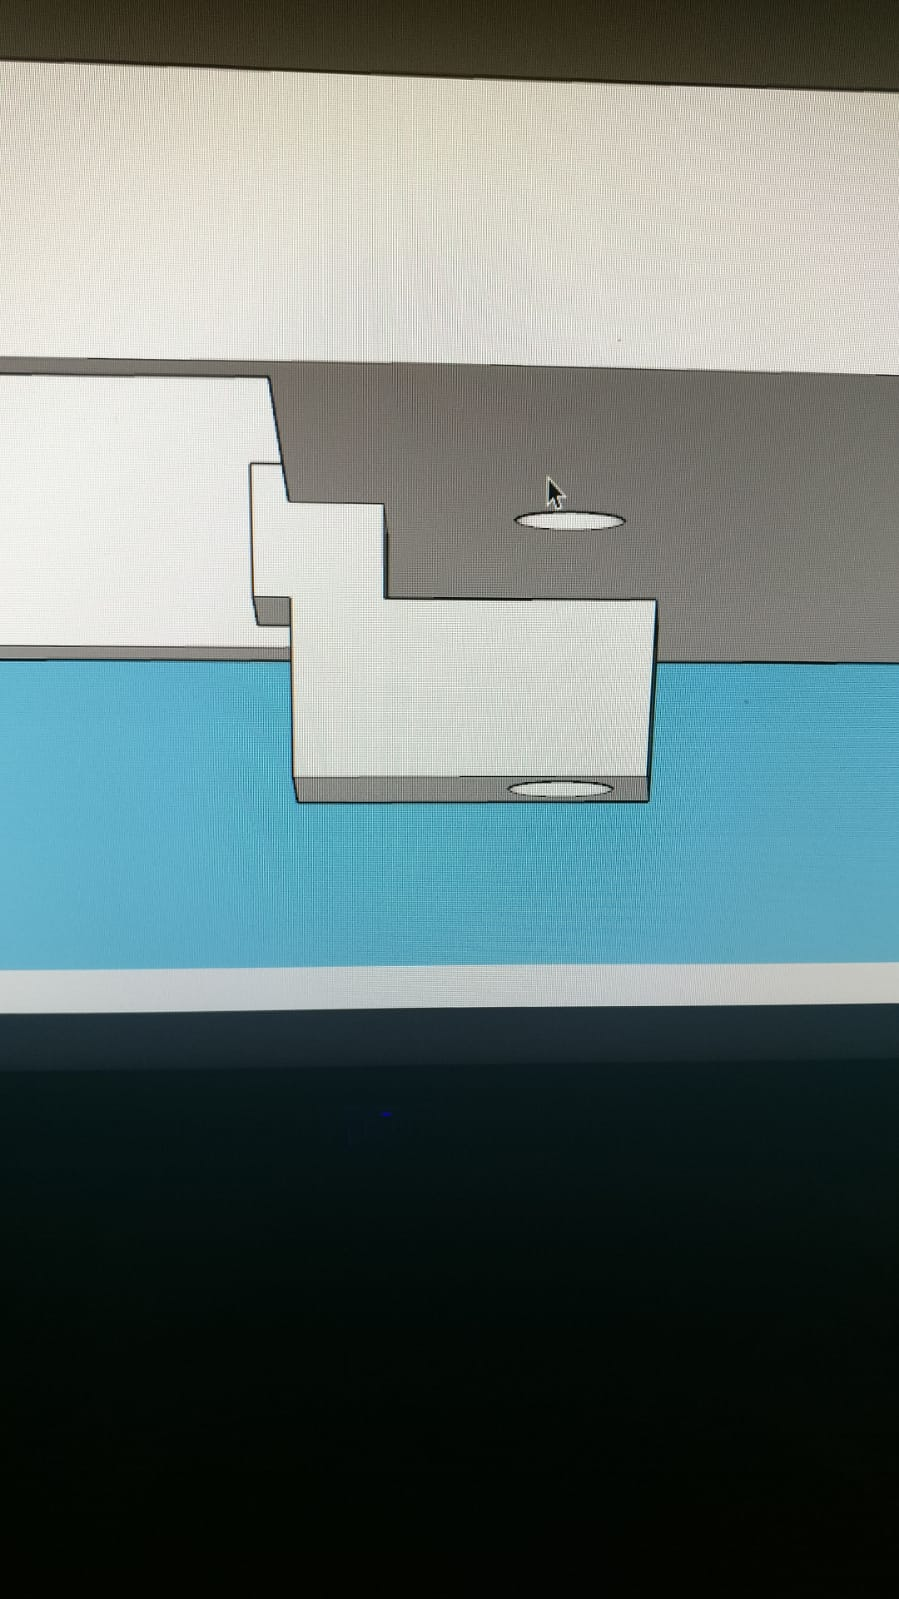
\includegraphics[
        width=0.5\linewidth,
    ]{imgs/new_fixture_upper.jpg}
    \caption{Neues Befestigungskonzept (obere Hälfte)}
    \label{fig-new-fixture-upper}
\end{center}
\end{figure}
\noindent
\begin{figure}[H]
\begin{center}
    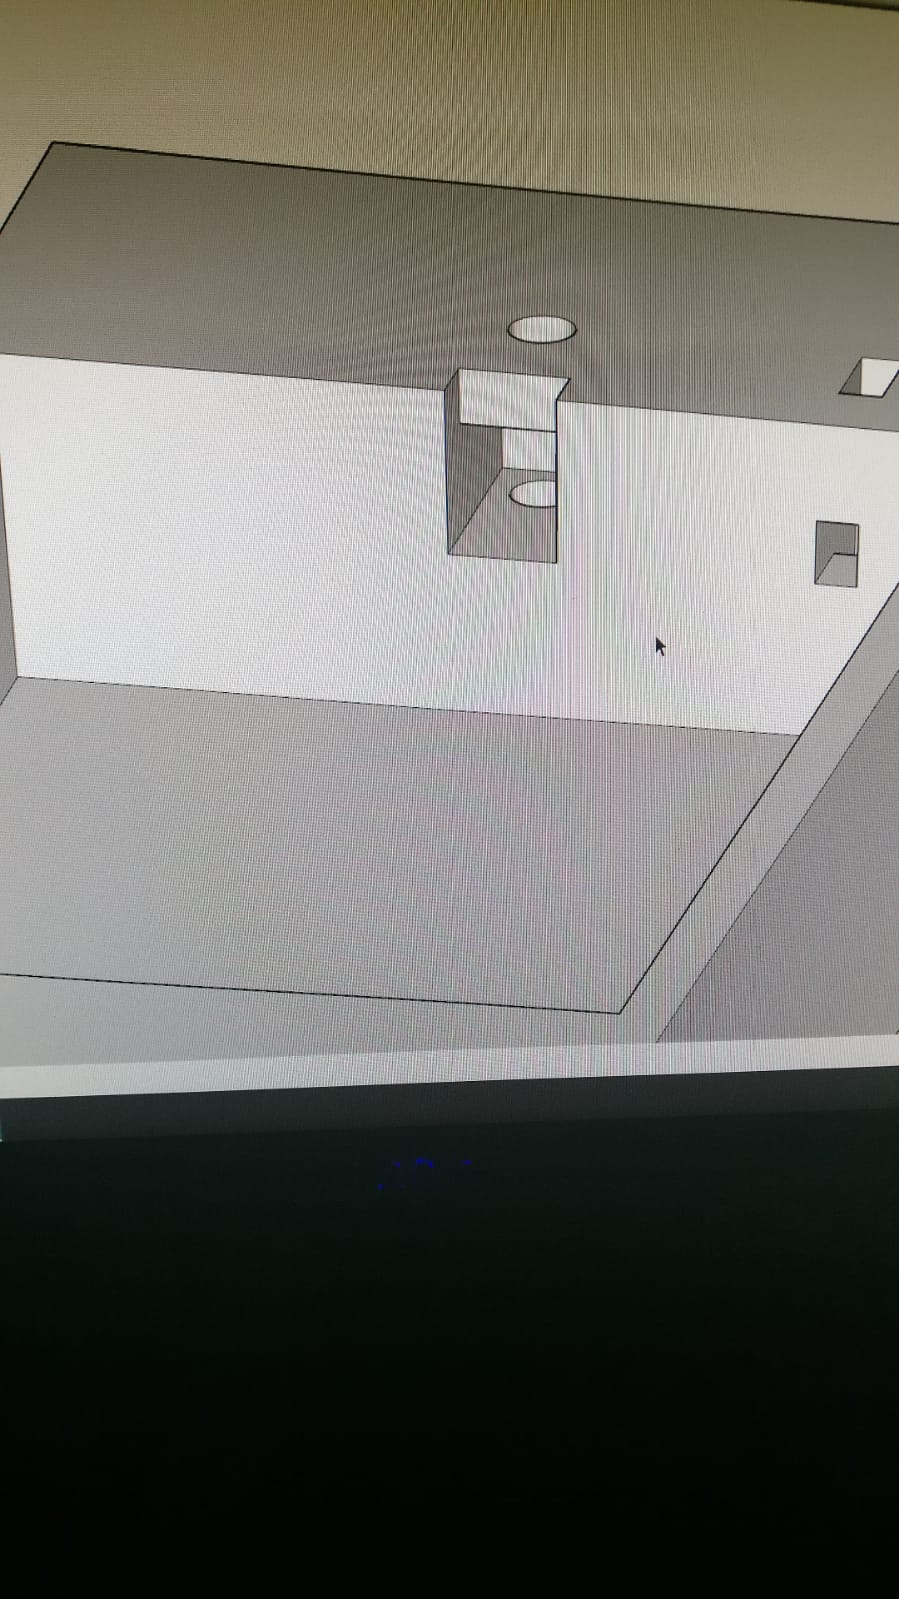
\includegraphics[
        width=0.5\linewidth,
    ]{imgs/new_fixture_lower.jpg}
    \caption{Neues Befestigungskonzept (untere Hälfte)}
    \label{fig-new-fixture-lower}
\end{center}
\end{figure}
\noindent 
Außerdem wurden die Aussparungen für Scheinwerfer und Hall-Sensor erweitert, 
um umständlichen Berechnungen und Probedrucken entgegn zu wirken.
\end{document}